\section{Theoretische Vorbereitung}
    %http://muenchuwe.com/nonhtml/papers/fest-25.pdf
    \subsection{Kristallstrukturen}
        Die meisten Festkörper lassen sich durch Kristallstrukturen beschreiben. Eine Kristallstruktur besteht
        dabei in der Regel aus einer endlichen Aneinanderreihung der sogenannten Elementarzelle. Die Elementarzelle ist
        jene Zelle, bestehend aus einer gruppe von atomen an ihren gitterpunkten, die durch lückenloses und translationssymetrisches aneinanderfügen das gitter Erzeugt. Die Elementarzelle
        lässt sich jedoch noch einmal aufteilen in die sogenannte Basis. Diese ist die kleinste gruppe Atome die
        sich in dem fraglichen Gitter wiederholt. Elementarzelle und Basiszelle können in manchen fällen äquivalent sein.
    \subsection{Gitterfehler}
        Innerhalb der gitter kann es zu abweichungen von der perfekten kristallinen struktur kommen, diese Gitterfehler lassen
        sich in verschiedene gruppen aufteilen
        \subsubsection*{0 Dimensionale Fehler}
            Punktdefekte beschreiben die veränderung von einzelnen atomen im gitter, dabei kann es vorkommen, das 
            einzelne gitterpunkte nicht besetzt sind und somit eine \textbf{Leerstelle} bilden.
            Alternativ kann es auch vorkommen das in einem gitter eine position von einem andersartigen atom besetzt wird,
            diese fehlstellen werden auch als \textbf{Substitutionsatome bezeichnet}.
            Zu guter letzt kann es auch vorkommen, dass gitterplätze besetzt sind die im regulären gitter gar nicht vorkommen,
            solche besetzungen bezeichnet man als \textbf{Zwischengitteratome}.\\
            Punktfehler lassen sich noch weiter differnzieren, da punktdefekte für diesen versuch jedoch keine besondere
            rolle spielen, möchten wir an dieser stelle auf fachlitteratur verweisen.
        \subsubsection*{1 Dimensionale Fehler}
            Linienfehler oder auch \textbf{Versetzungen} sind hier von besonderem interesse. Linienfehler haben 
            großen einfluss auf die mechanischen eigenschaften eines festkörpers, diese eigenschaft dient im späteren verlauf
            als nachweismethode solcher fehler im kristall. Eine Veretzung ist im allgemeinen eine Störung des periodischen gitters, 
            die sich, anders als Punktdefekte, entlang einer linie im kristall fortsetzt. Sie enstehen durch krafteinwirkungen auf das gitter,
            durch Eigenspannung, beim wachstum oder durch äussere kräfte bei plastischer deformation.\\
            Bei versetzung wird in der regel zwischen Stufenversetzungen und Schraubenversetzungen unterschieden,
            sie werden durch den Burgers vektor definiert, der im nächsten abschnitt nocheinmal näher erklärt wird.
            Bei Stufenversetzung stehen der Burgersvektor und die versetzungseben senkrecht zueinander.
            \begin{figure}[H]
                \centering
                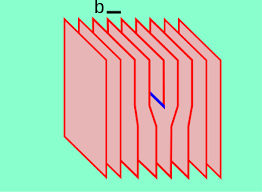
\includegraphics[width=0.5\textwidth]{Images/Stufenversetzung}
                \caption{Schematische darstellung einer Stufenversetzung}
            \end{figure}
            Bei Schraubenversetzungen hingegen stehen Burgersvektor und Burgersvektor parralel zueinander.
            \begin{figure}[H]
                \centering
                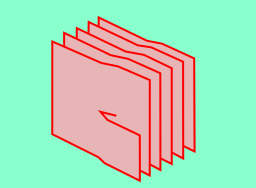
\includegraphics[width=0.5\textwidth]{Images/Schraubenversetzung}
                \caption{Schematische darstellung einer Schraubenversetzung}
            \end{figure}
        \subsubsection*{2 Dimensionale Fehler}
            Eine weiter gruppe gitterfehler sind die \textbf{Flächenfehler}. Den wohl simpelsten flächenfehler
            stellt die oberfläche eines Kristalls dar, da dort eine unterbrechung der periodizität und translationssymetrie vorliegt.
            Ein anderer flächenfehler ist die sogenannte \textbf{Kleinwinkelkorngrenze}. An Kleinwinkelkorngrenzen kommen zwei 
            Bereiche des Kristallgitter mit verschiedener räumlicher Orientierung zusammen, diese grenzen lassen sich anhand ihrer winkel
            anschließend noch in Kleinwinkelkorngrenzen und großwinkelkorngrenzen unterteilen.
            \begin{figure}[H]
                \centering
                \includegraphics[width=0.5]{Images/kleinwinkelkorngrenze}
                \caption{Schematische Darstellung einer Kleinwinkelkorngrenze}
            \end{figure}
            Sogennante \textbf{Stapelfehler} bezeichnen fehler in der Stapelreihenfolge in einem kristallgitter. Solche fehler in der periodizität
            kann zu bildungen von Kleinwinkelkorngrenzen führen.
            Weitere 2 Dimensionale Fehler sind die Antiphasengrenze und die Zwillingsgrenze sowie Domänenwände, diese tragen jedoch nicht
            zu diesem Versuch bei und werden daher hier nicht näher beschrieben.
        \subsubsection*{3 Dimensionale Fehler}
            Die letzte gruppe ist die gruppe der 3 dimensionalen fehler, oder auch Volumenfehler. Sie bezeichnen einbindungen vollständig verschiedener stoffe innerhalb der ursprünglichen
            Krsitallstruktur, so bezeichnen \textbf{Poren} Hohlräume im Kristall die mit gas oder flüssigkeit gefüllt sind wohingegen
            \textbf{Einschlüsse} eingeschlossen festkörper beschreiben.
            Diese fehler sind in der regel Makroskopischer größenordnung, führen jedoch an ihren grenzen zum ursprünglichen krsitallgitter
            zu einer reihe niederdimensionaler gitterfehler.

    \subsection{Burgers Vektor}
            
    \subsection{Ätzgrübchen}

    \subsection{Lithiumflourid}